%=========================================================
% RTL Files and Structure of SoC
%=========================================================
\section{RTL Files and Structure of SoC}

RTL files of mmRISC-1 tiny SoC are shown in Table \ref{tb:CHIPRTLFILES}, and the corresponding RTL structure is shown in Figure \ref{fig:CHIPRTLSTRUCTURE}.

\begin{table}[H]
    \begin{adjustbox}{scale={0.6}{0.7}}
    \textsf{
    \begin{tabular}{|L{8cm}{6cm}{t}|L{7cm}{4cm}{t}|L{10cm}{9cm}{t}|L{3cm}{2cm}{t}|}
        \hline
        %-------------------------------------
        \rowcolor{LightPurple}
        \textbf{Directory} &
        \textbf{File Name} &
        \textbf{Description} &
        \textbf{Note}
        \nextRow \hline
        %-------------------------------------
        verilog/common &
        defines\_chip.v &
        Definitions and Configurations for Chip &
        ~
        \nextRow \hline
        %-------------------------------------
        verilog/chip &
        chip\_top\_wrap.v &
        Wrap of Top Layer of Chip &
        ~
        \nextRow \hline
        %-------------------------------------
        verilog/chip & 
        chip\_top.v &
        Top Layer of Chip &
        ~
        \nextRow \hline
        %-------------------------------------
        verilog/cjtag &
        cjtag\_2\_jtag.v &
        Converter from cJTAG to JTAG &
        ~
        \nextRow \hline
        %-------------------------------------
        verilog/cjtag &
        cjtag\_adapter.v &
        cJTAG Adapter (JTAG → cJTAG) &
        ~
        \nextRow \hline
        %-------------------------------------
        verilog/ahb\_matrix &
        ahb\_top.v &
        AHB Bus Matrix Top Layer &
        ~
        \nextRow \hline
        %-------------------------------------
        verilog/ahb\_matrix &
        ahb\_master.v &
        AHB Bus Matrix Master Port &
        ~
        \nextRow \hline
        %-------------------------------------
        verilog/ahb\_matrix &
        ahb\_interconnect.v &
        AHB Bus Matrix Interconnect &
        ~
        \nextRow \hline
        %-------------------------------------
        verilog/ahb\_matrix &
        ahb\_arb.v &
        AHB Bus Matrix Arbiter &
        ~
        \nextRow \hline
        %-------------------------------------
        verilog/ahb\_matrix &
        ahb\_slave.v &
        AHB Bus Matrix Slave Port &
        ~
        \nextRow \hline
        %-------------------------------------
        verilog/ram &
        ram.v &
        RAM for Instruction and Data Memory &
        ~
        \nextRow \hline
        %-------------------------------------
        verilog/ram &
        ram\_fpga.v &
        RAM for Instruction for FPGA with Initial Data &
        ~
        \nextRow \hline
        %-------------------------------------
        fpga &
        RAM128KB\_DP.v &
        Block RAM IP for ram\_fpga.v &
        ~
        \nextRow \hline
        %-------------------------------------
        fpga &
        RAM128KB\_DP.mif &
        Block RAM Initial Data &
        ~
        \nextRow \hline
        %-------------------------------------
        verilog/ahb\_sdram/logic &
        ahb\_lite\_sdram.v &
        Simple SDRAM Interface \lb
        (for 64MB : 32M x 16bits) &
        Zhelnio
        \nextRow \hline
        %-------------------------------------
        verilog/ahb\_sdram/model &
        sdr.v &
        External SDRAM Model for Test Bench &
        \setMultiRow{2}{Micron}
        \nextRow \cline{1-3}
        %-------------------------------------
        verilog/ahb\_sdram/model &
        sdr\_parameters.vh &
        External SDRAM Model Parameters for sdr.v &
        ~
        \nextRow \hline
        %-------------------------------------
        verilog/int\_gen &
        int\_gen.v &
        Interrupt Generator &
        ~
        \nextRow \hline
        %-------------------------------------
        verilog/uart &
        uart.v &
        UART Top Layer &
        ~
        \nextRow \hline
        %-------------------------------------
        verilog/uart/sasc/trunk/rtl/verilog &
        sasc\_top.v &
        Simple Asynchronous Serial Controller \lb Top Layer&
        \setMultiRow{4}{OpenCores \lb SASC IP}
        \nextRow \cline{1-3}
        %-------------------------------------
        verilog/uart/sasc/trunk/rtl/verilog &
        sasc\_fifo4.v &
        Simple Asynchronous Serial Controller \lb FIFO &
        ~
        \nextRow \cline{1-3}
        %-------------------------------------
        verilog/uart/sasc/trunk/rtl/verilog &
        sasc\_brg.v &
        Simple Asynchronous Serial Controller \lb Baud Rate Generator &
        ~
        \nextRow \cline{1-3}
        %-------------------------------------
        verilog/uart/sasc/trunk/rtl/verilog &
        timescale.v &
        Simple Asynchronous Serial Controller \lb Time Scale &
        ~
        \nextRow \hline
        %-------------------------------------
        verilog/i2c &
        i2c.v &
        I2C Top Layer &
        ~
        \nextRow \hline
        %-------------------------------------
        verilog/i2c/i2c/trunk/rtl/verilog &
        i2c\_master\_top.v &
        I2C Master Controller Top Level &
        \setMultiRow{4}{OpenCores \lb I2C IP}
        \nextRow \cline{1-3}
        %-------------------------------------
        verilog/i2c/i2c/trunk/rtl/verilog &
        i2c\_master\_byte\_ctrl.v &
        I2C Master Controller Byte Control Block &
        ~
        \nextRow \cline{1-3}
        %-------------------------------------
        verilog/i2c/i2c/trunk/rtl/verilog &
        i2c\_master\_bit\_ctrl.v &
        I2C Master Controller Bit Control Block &
        ~
        \nextRow \cline{1-3}
        %-------------------------------------
        verilog/i2c &
        i2c\_slave\_model.v &
        I2C Slave Model for Test Bench &
        ~
        \nextRow \hline
        %-------------------------------------
        verilog/spi &
        spi.v &
        SPI Top Layer &
        ~
        \nextRow \hline
        %-------------------------------------
        verilog/spi/simple\_spi/trunk/rtl/verilog &
        simple\_spi\_top.v &
        Simple SPI Top Level &
        \setMultiRow{2}{OpenCores \lb Simple SPI}
        \nextRow \cline{1-3}
        %-------------------------------------
        verilog/spi/simple\_spi/trunk/rtl/verilog &
        fifo4.v &
        Simple SPI FIFO Block &
        ~
        \nextRow \hline
        %-------------------------------------
        verilog/port &
        port.v &
        GPIO &
        ~
        \nextRow \hline
        %-------------------------------------
        fpga &
        PLL.v &
        PLL IP for FPGA \lb
        (50MHz –> 20MHz and 16.667MHz) &
        ~
        \nextRow \hline
        %-------------------------------------
        mmRISC-1 RTLs &
        Table \ref{tb:RTLFILES} &
        mmRISC-1 Block &
        ~
        \nextRow \hline
        %-------------------------------------
    \end{tabular}
    }
    \end{adjustbox}
    \caption{RTL Files of SoC}
    \label{tb:CHIPRTLFILES}
\end{table}

Basically, the debug interface is 4-wire JTAG, but you can use 2-wire cJTAG (Compact JTAG) instead. To select the debug interface from either 4-wire JTAG or 2-wire cJTAG, please use a define switch "\textasciigrave define ENABLE\_CJTAG" in verilog/common/defines\_core.v". When using 4-wire JTAG, please comment out the \textasciigrave define statement, whereas when using 2-wire cJTAG, leave the \textasciigrave define statement as active. The chip top RTL is surrounded by chip\_top\_wrap.v as shown in Figure \ref{fig:cJTAG_FPGA}. When selecting cJTAG interface, the cjtag\_adapters.v is included in the layer of chip\_top\_wrap.v, and cjtag\_2\_jtag.v is included in the layer of chip\_top.v. Even when selecting JTAG interface, to make the structure of chip top same as cJTAG version the chip top layer is also chip\_top\_wrap.v and unnecessary cJTAG related logics are eliminated by the \textasciigrave define switch.

\begin{figure}[H]
    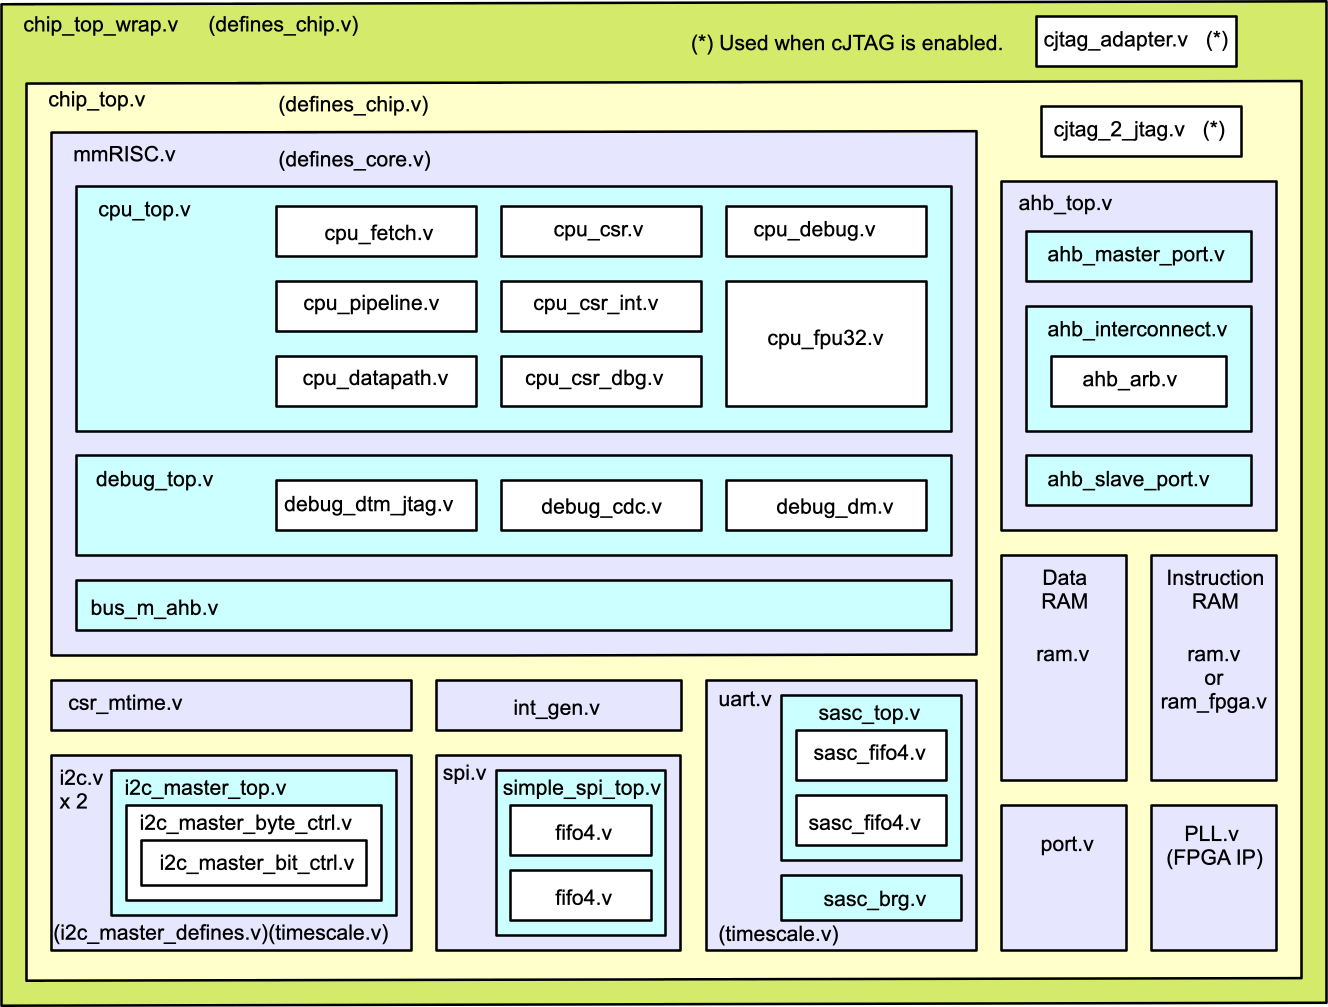
\includegraphics[width=1.0\columnwidth]{./Figure/CHIPRTLStructure.png}
    \caption{Structure of RTL Files of SoC}
    \label{fig:CHIPRTLSTRUCTURE}
\end{figure}

